\documentclass{article}
\usepackage{amsmath}
\usepackage{amssymb}
\usepackage{fancyhdr}
\usepackage[utf8]{inputenc}
\usepackage{tcolorbox}
\usepackage[left=1in, right=1in, top=1.5in, bottom=1in]{geometry}
\usepackage{tikz}
\usepackage{enumerate}
\usepackage{enumitem}
\usepackage{pgfplots}
\usepackage{ragged2e}
\usepackage{tabularx}
\usepackage{array}
\usepackage{mdframed}
\pgfplotsset{compat=1.18}
\begin{document}
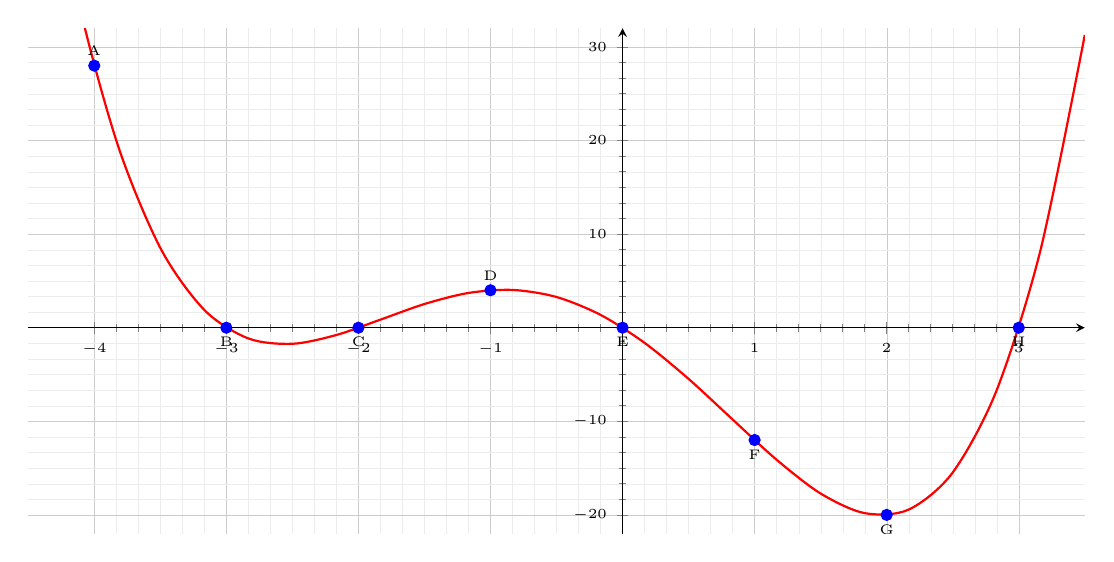
\begin{tikzpicture}
\begin{axis}[
    % Set the overall dimensions of the plot area
    height=8cm, 
    width=15cm,  
    % Set the domain and range for the axes
    xmin=-4.5, xmax=3.5,
    ymin=-22, ymax=32,
    % Manually set the tick marks
    xtick={-4,-3,-2,-1,0,1,2,3},
    ytick={-20,-10,0,10,20,30},
    % Add 5 minor lines between each major tick on both axes
    minor x tick num=5,
    minor y tick num=5,
    % This command draws both major and minor grid lines
    grid=both,
    major grid style={line width=.1pt,draw=gray!40},
    minor grid style={line width=.1pt,draw=gray!15},
    % Axis and label styling
    axis lines=middle,
    tick label style={font=\tiny},
    xlabel style={at={(current axis.right of origin)}, anchor=west},
    ylabel style={at={(current axis.above origin)}, anchor=south},
    axis line style={-stealth},
]

\addplot[domain=-4.5:3.5, smooth, thick, red] {(1/2)*(x)*(x-3)*(x+3)*(x+2)};
\draw[fill=blue, draw=blue] (-4, 28)   circle (2pt) node[above, font=\tiny] {A};
\draw[fill=blue, draw=blue] (-3, 0)    circle (2pt) node[below, font=\tiny] {B};
\draw[fill=blue, draw=blue] (-2, 0)    circle (2pt) node[below, font=\tiny] {C};
\draw[fill=blue, draw=blue] (-1, 4)    circle (2pt) node[above, font=\tiny] {D};
\draw[fill=blue, draw=blue] (0, 0)     circle (2pt) node[below, font=\tiny] {E};
\draw[fill=blue, draw=blue] (1, -12)   circle (2pt) node[below, font=\tiny] {F};
\draw[fill=blue, draw=blue] (2, -20)   circle (2pt) node[below, font=\tiny] {G};
\draw[fill=blue, draw=blue] (3, 0)     circle (2pt) node[below, font=\tiny] {H};
\end{axis}
\end{tikzpicture}
\end{document}